\chapter{隐私保护密度聚类方法研究}
\section{引言}
% 1.说明隐私保护k-means研究存在的问题
海量可获取的数据以及云计算提供的计算能力驱动机器学习的快速发展。有监督学习例如神经网络,使用带标签的数据来训练具有识别能力的模型。与之相反的是无监督学习,没有训练模型的过程,旨在从未标记的数据中发现未知的模式和特征。聚类是一种广泛使用的无监督机器学习工具,能够将相似的数据划分到同一个集合中。实际应用中,聚类常用于许多数据安全极为重要的领域,例如商业数据分析,市场数据挖掘以及医院病理信息分析等。上述场景中,数据一旦泄露会造成极大经济损失。

目前,已有许多关于隐私保护聚类方案的研究,其中数量最多的是与k-means相关的研究ref-sok。然而k-means聚类过程相对比较简单,并且只能检测到凸型簇,因此适用数据集类型极为受限。此外,簇的数量$k$必须要根据专业领域知识提前给出,如果只了解数据集的子集难以确定$k$的值。同时,k-means聚类不包含噪声的概念,并且聚类的结果对异常值非常敏感因为每一个输入都要被划分到某一个簇中。因此,即便某个输入不属于任何一个簇,它都会被划分到距离最近的簇,影响该簇的中心位置(簇中所有数据的平均值)。

% 2.隐私保护dbscan的好处
为了解决上述隐私保护方案中存在的问题,这里我们引入对隐私保护density-based spatial clustering of applications with noise(dbscan)的研究。dbscan是一种由ref-dbscan-ester20提出的更加灵活的聚类算法,能够检测到任意形状的簇。此外,簇的数量是根据数据集的特点灵活产生的,无需人工确定。该算法对异常值不敏感,会将其标记为噪声。本章首先提出了方案一,一种安全高效的隐私保护dbscan方案,该方案针对明文算法进行改进以适应安全计算的特点,将复杂度降低为$O(n^2)$,显著降低聚类所需时间。

传统dbscan方案存在数据划分结果不稳定的问题,即最终划分结果取决于算法运行中数据遍历的顺序,将数据打乱后重新进行聚类,同一个点可能会被划分到不同的簇中。为了解决该问题,在ref-redbscan论文思想的基础上,我们在方案二中提出了改进的隐私保护dbscan,以获取稳定的聚类结果。

尽管dbscan具有诸多优点,其聚类过程涉及两个重要参数MinPts和Eps,这两个参数的取值与数据分布密切相关,通常需要人工分析后给出。为解决该问题,在论文ref-dbhc的基础上,我们在方案三中提出了基于dbscan的隐私保护层次聚类,借助k近邻算法和k线图来决定聚类参数,并进行多轮聚类来适应不同密度的簇。
% 3.本章组织结构
本章的组织结构如下:第\ref{s4-yubei}节介绍了dbscan的相关内容。第\ref{s4-wenti}节中描述了系统模型、安全模型以及设计目标。第\ref{s4-subpro}节中增加了一些基于秘密共享的隐私保护计算模块。第\ref{s4-t1}节对隐私保护dbscan方案进行了详细介绍。第\ref{s4-t2}节中提出了方案二改进的隐私保护dbscan方案。第\ref{s4-t3}节中阐述了基于dbscan的隐私保护层次聚类方案。第\ref{s4-lilun}节中从理论上分析了方案的正确性和安全性。第\ref{s4-shiyan}节中对方案进行了实验评估。最后,在\ref{s4-xiaojie}节对本章进行了总结。

\section{预备知识}
\label{s4-yubei}
\subsection{DBSCAN}
Density-based Spatial Clustering of Applications with Noise(DBSCAN)是一种基于密度的聚类算法,在密集区域聚集在一起的数据点被划分到同一个簇中,稀疏区域的数据被标记为噪声。算法要求两个重要参数:
\begin{itemize}
	\item $\epsilon$: 确定两个点被视为相邻的最大距离
	\item MinPts: 确定领域内至少包含多少点才能构成一个簇
\end{itemize}

DBSCAN围绕每个数据点以$\epsilon$为半径构建圈,并将其划分为核心点、边界点以及噪声点。若圈内不包含任何点,则认为是噪声点。若数据点圈内包含点的数量至少为MinPts个,则认为是核心点,否则为边界点。围绕上述定义展开,DBSCAN还包含如下概念:

假设样本集为$D=(x_1,x_2,...,x_m)$:
\begin{itemize}
	\item 密度直达: 若$ x_i $位于$ x_j $的$ \epsilon- $邻域内,且$ x_j $为核心对象,则称$ x_i $由$ x_j $密度直达,反之不一定成立。
	\item 密度可达: 对于$ x_i $和$ x_j $,若存在样本序列$ p_1,p2,...,p_t $,满足$ p_1=x_i,p_T=x_j $,且$ p_{t+1} $由$ p_t $密度直达,则称$ x_j $由$ x_i $密度可达。
	\item 密度相连: 对于$ x_i $和$ x_j $,如果存在核心点$ x_k $,使得$ x_i $和$ x_j $均由$ x_k $密度可达,则称$ x_i $和$ x_j $密度相连。
\end{itemize}


下面我们具体阐述DBSCAN聚类算法的流程:

\begin{enumerate}
	\item 初始化核心点集合$ \Omega = \varnothing  $,初始化簇数量$ k=0 $,初始化未访问点集合$ \Gamma = D $,簇划分$ C=\varnothing $
	\item 遍历所有点$ i=1,2,...,m $,按如下方式找到所有核心点:
	\begin{enumerate}
	\item 计算距离,找到样本$ x_i $的$ \epsilon- $邻域内所有点集合$ N_{\epsilon}(x_i) $
	\item 如果集合包含数据点个数满足$ |N_{\epsilon}(x_i)| \geq MinPts $,将$ x_i $加入核心点集合:$ \Omega = \Omega \cup \{x_j\} $
	\end{enumerate}	
	\item 若$ \Omega = \varnothing $,则算法结束,否则转入步骤4
	\item 在$ \Omega $中,随机选择一核心点$ o $,初始化当前簇包含核心点集合$ \Omega_{c}=\{o\} $,簇序号为$ k=k+1 $,当前簇包含点集合$ C_k=\{o\} $,更新未访问样本集合$ \Gamma = \Gamma - \{o\} $
	\item 若$ \Omega_{cur} = \varnothing $, 则簇$ C_k $聚类完毕,更新簇集合$ C=\{C_1,C_2,...,C_k\} $,更新核心点集合$ \Omega = \Omega - C_k $
	\item 从$ \Omega_{cur} $中取出一个核心点$ o' $,通过邻域距离$ \epsilon $找到所有$ \epsilon- $邻域子集$ N_{\epsilon}(o')  $,令$ \Delta = N_{\epsilon}(o') \cap \Gamma $,更新当前簇包含点集合$ C_k = C_k \cup \Delta $,更新未访问点集合$ \Gamma = \Gamma - \Delta $,更新$ \Omega_{cur} = \Omega_{cur}\cup(\Delta\cap\Omega)-o' $,转入步骤5
	\item 输出结果为: 簇划分$ C=\{C_1,C_2,...,C_k\} $
\end{enumerate}
%来源为https://www.cnblogs.com/pinard/p/6208966.html

DBSCAN能够应用于任意维度的数据集。铭文上最坏情况下的复杂度为$ O(n^2) $,其中$ n $为数据的数量。
\section{问题描述}
\label{s4-wenti}
\subsection{系统模型}
\begin{figure}[htbp]
	\centering
	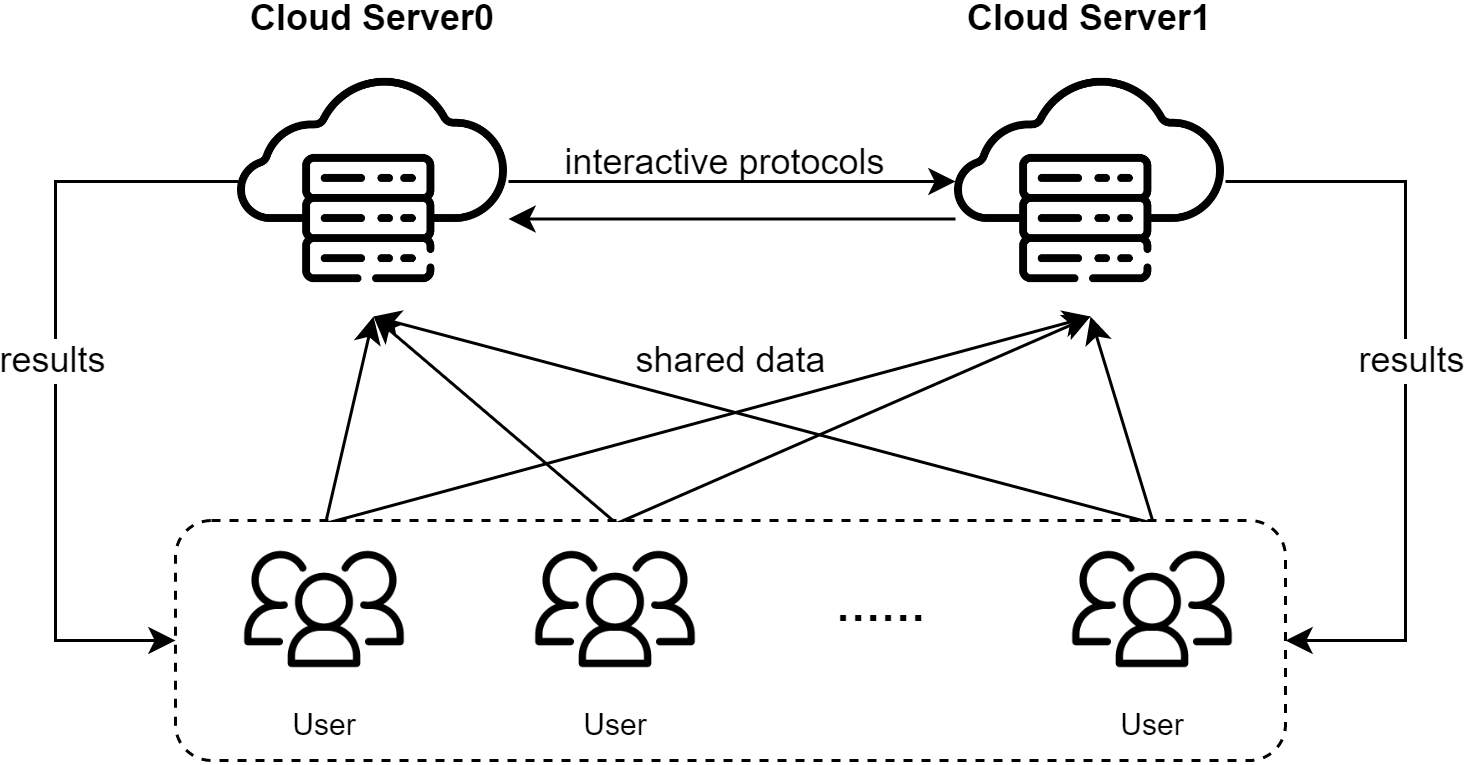
\includegraphics[width=3in]{img/ch4-sysmod.png}%width=\linewidth
	\caption{System Model}
	\label{s4-sysmod}
\end{figure}
如图\ref{s4-sysmod}琐事,我们的系统由两个部分组成:服务器短和用户端。与图\ref{sys model}类似,服务器端为两个云服务器,获取用户数据后执行协议,最后分发结果。不同的是,\ref{sys model}中用户为某一个持有全部明文数据的组织机构,本方案系统模型中的用户即可以与
\subsection{安全模型}

\subsection{设计目标}
\section{基于秘密共享的隐私保护计算模块}
\label{s4-subpro}
\section{隐私保护dbscan}
\label{s4-t1}
\section{改进的隐私保护dbscan}
\label{s4-t2}
\section{基于dbscan的层次聚类}
\label{s4-t3}
\section{理论分析}
\label{s4-lilun}
\section{实验评估}
\label{s4-shiyan}
\section{本章小结}
\label{s4-xiaojie}